\begin{figure}[htbp]
    \centering
    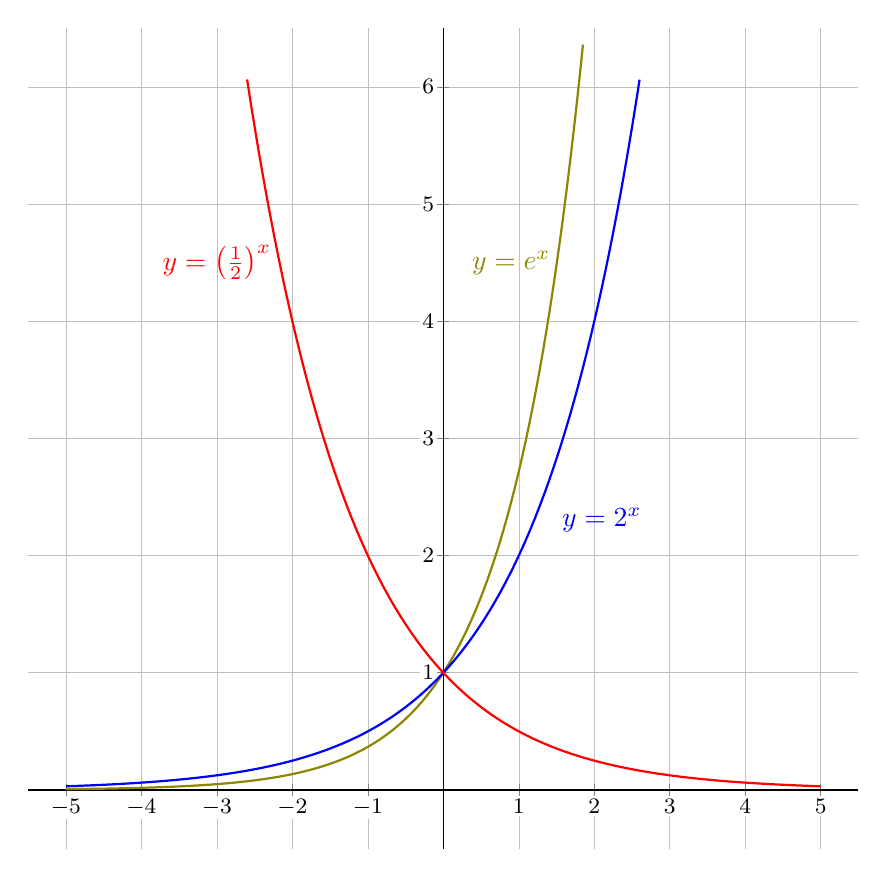
\begin{tikzpicture}
        % --- (giữ nguyên code vẽ hình của bạn ở đây) ---
        \begin{axis}[
            width=1\textwidth,
            height=12cm,
            axis lines=middle,
            grid=major,
            grid style={line width=.1pt, draw=gray!20},
            major grid style={line width=.2pt,draw=gray!50},
            xmin=-5.5, xmax=5.5,
            ymin=-0.5, ymax=6.5,
            xtick={-5, -4, -3, -2, -1, 0, 1, 2, 3, 4, 5},
            ytick={1, 2, 3, 4, 5, 6},
            ticklabel style={font=\footnotesize, fill=white, inner sep=1pt},
            axis line style={-},
            smooth,
            no marks,
            samples=200,
        ]

        % Vẽ đồ thị y = e^x
        \addplot[olive, thick, domain=-5:1.85] {exp(x)}; % Đổi màu blackgreen thành olive cho chuẩn
        \node[olive] at (axis cs:0.9, 4.5) {$y=e^x$};

        % Vẽ đồ thị y = 2^x
        \addplot[blue, thick, domain=-5:2.6] {2^x};
        \node[blue] at (axis cs:2.1, 2.3) {$y=2^x$};

        % Vẽ đồ thị y = (1/2)^x
        \addplot[red, thick, domain=-2.6:5] {(1/2)^x};
        \node[red] at (axis cs:-3, 4.5) {$y=\left(\frac{1}{2}\right)^x$};

        \end{axis}
    \end{tikzpicture}
    \caption{Đồ thị của một số hàm mũ.\footnotemark} % <-- SỬA Ở ĐÂY: Dùng \footnotemark
    \label{fig:plot_exp_functions}
\end{figure}
\footnotetext{Chú ý dáng điệu và sự khác nhau khi cơ số lớn hơn 1 và bé hơn 1.} % <-- SỬA Ở ĐÂY: Dùng \footnotetext ngay sau figure